\documentclass{beamer}
\usepackage[utf8]{inputenc}
\usepackage[english]{babel}
\usepackage{helvet}
\usepackage[T1]{fontenc}
\usepackage{textcomp}
\usepackage[inline]{asymptote}
\usepackage{slide_helper}
\usepackage{tikz}
\usetikzlibrary{shapes.geometric, arrows}
\usepackage{pgfplots}
\pgfplotsset{compat=1.5} 
\usepgfplotslibrary{statistics}
\usetikzlibrary{external}
\tikzexternalize%

\title[MA205 - Section 2.1]{Examining Numerical Data}

\begin{document}
\begin{frame}
\titlepage
\end{frame}

\begin{frame}
\begin{example}
Let us consider a scatterplot of borrowers total income and the loan amount from the \texttt{loan50} data set.

\only<1| handout:0>{
\begin{center}
\begin{tikzpicture}
\tikzstyle{every pin}=[
fill=white,
draw=black,
font=\tiny,
]
\pgfkeys{/pgf/number format/.cd,
fixed,
precision=999,
set thousands separator={},
1000 sep in fractionals=false,
}
\begin{axis}[
clip mode=individual,
clip marker paths=true,
width=10cm,
height=5cm,
xlabel={Total Income},
ylabel={Loan Amount},
grid=major,
%ymajorgrids=true,
%xmajorgrids=true,
%enlarge x limits=false,
%enlarge y limits=false,
%xticklabel style={/pgf/number format/.cd,fixed,precision=0},
xticklabel=\$\pgfmathprintnumber{\tick}k,,
yticklabel=\$\pgfmathprintnumber{\tick}k,,
xtick={0, 50000, 100000, 150000, 200000, 250000, 300000},
ytick={0, 10000, 20000, 30000, 40000},
scaled x ticks=base 10:-3,
xtick scale label code/.code={},
scaled y ticks=base 10:-3,
ytick scale label code/.code={},
ymin=-5,
ymax=35000,
xmin=-5,
xmax=325000,
scatter/use mapped color={
%draw=mapped color,
fill=black,
},
]
\addplot [scatter, only marks, blue!50!black, scatter src=y, mark size=0.8pt] 
table [y=loan_amount, x=total_income, col sep=comma] {loan50.csv};
\end{axis}
\end{tikzpicture}
\end{center}
}
\only<2->{
\begin{center}
\begin{tikzpicture}
\tikzstyle{every pin}=[
fill=white,
draw=black,
font=\tiny,
]
\pgfkeys{/pgf/number format/.cd,
fixed,
precision=999,
set thousands separator={},
1000 sep in fractionals=false,
}
\begin{axis}[
clip mode=individual,
clip marker paths=true,
width=10cm,
height=5cm,
xlabel={Total Income},
ylabel={Loan Amount},
grid=major,
%ymajorgrids=true,
%xmajorgrids=true,
%enlarge x limits=false,
%enlarge y limits=false,
%xticklabel style={/pgf/number format/.cd,fixed,precision=0},
xticklabel=\$\pgfmathprintnumber{\tick}k,,
yticklabel=\$\pgfmathprintnumber{\tick}k,,
xtick={0, 50000, 100000, 150000, 200000, 250000, 300000},
ytick={0, 10000, 20000, 30000, 40000},
scaled x ticks=base 10:-3,
xtick scale label code/.code={},
scaled y ticks=base 10:-3,
ytick scale label code/.code={},
ymin=-5,
ymax=35000,
xmin=-5,
xmax=325000,
scatter/use mapped color={
%draw=mapped color,
fill=black,
},
]
\addplot [scatter, only marks, red, scatter src=y, mark size=1.0pt,, scatter/use mapped color={fill=red,}]
table [y=loan_amount, x=total_income, col sep=comma, x expr={\thisrow{total_income} / (\thisrow{total_income} <= 100000)}] {loan50.csv};
\addplot [scatter, only marks, blue!50!black, scatter src=y, mark size=0.8pt]
table [y=loan_amount, x=total_income, col sep=comma, x expr={\thisrow{total_income} / (\thisrow{total_income} > 100000)}] {loan50.csv};
\addplot [mark size=0pt, red, line width=0.5pt] coordinates {(100000,0) (100000,35000)};
\end{axis}
\end{tikzpicture}
\end{center}
}\pause

We can see that the many of borrowers earn \$100,000 a year or less.
\end{example}
\end{frame}

\begin{frame}
\begin{example}
Let us consider a scatterplot of borrowers total income and the loan amount from the \texttt{loan50} data set.

\only<1| handout:0>{
\begin{center}
\begin{tikzpicture}
\tikzstyle{every pin}=[
fill=white,
draw=black,
font=\tiny,
]
\pgfkeys{/pgf/number format/.cd,
fixed,
precision=999,
set thousands separator={},
1000 sep in fractionals=false,
}
\begin{axis}[
clip mode=individual,
clip marker paths=true,
width=10cm,
height=5cm,
xlabel={Poverty Rate},
ylabel={Median Household Income},
grid=major,
%ymajorgrids=true,
%xmajorgrids=true,
%enlarge x limits=false,
%enlarge y limits=false,
%xticklabel style={/pgf/number format/.cd,fixed,precision=0},
xticklabel=\pgfmathprintnumber{\tick}\%,
yticklabel=\$\pgfmathprintnumber{\tick}k,
xtick={0, 10, 20, 30, 40, 50},
ytick={0, 20000, 40000, 60000, 80000, 100000, 120000},
%scaled x ticks=base 10:-3,
%xtick scale label code/.code={},
scaled y ticks=base 10:-3,
ytick scale label code/.code={},
ymin=-5,
ymax=125000,
xmin=-5,
xmax=60,
scatter/use mapped color={
%draw=mapped color,
fill=black,
},
]
\addplot [scatter, only marks, blue!50!black, scatter src=y, mark size=0.3pt] 
table [y=median_hh_income, x=poverty, col sep=comma,ignore chars={N,A}] {county.csv};
\end{axis}
\end{tikzpicture}
\end{center}
}
\only<2->{
\begin{center}
\begin{tikzpicture}
\tikzstyle{every pin}=[
fill=white,
draw=black,
font=\tiny,
]
\pgfkeys{/pgf/number format/.cd,
fixed,
precision=999,
set thousands separator={},
1000 sep in fractionals=false,
}
\begin{axis}[
clip mode=individual,
clip marker paths=true,
width=10cm,
height=5cm,
xlabel={Poverty Rate},
ylabel={Median Household Income},
grid=major,
%ymajorgrids=true,
%xmajorgrids=true,
%enlarge x limits=false,
%enlarge y limits=false,
%xticklabel style={/pgf/number format/.cd,fixed,precision=0},
xticklabel=\pgfmathprintnumber{\tick}\%,
yticklabel=\$\pgfmathprintnumber{\tick}k,
xtick={0, 10, 20, 30, 40, 50},
ytick={0, 20000, 40000, 60000, 80000, 100000, 120000},
%scaled x ticks=base 10:-3,
%xtick scale label code/.code={},
scaled y ticks=base 10:-3,
ytick scale label code/.code={},
ymin=-5,
ymax=125000,
xmin=-5,
xmax=60,
scatter/use mapped color={
%draw=mapped color,
fill=black,
},
]
\addplot [scatter, only marks, blue!50!black, scatter src=y, mark size=0.3pt] 
table [y=median_hh_income, x=poverty, col sep=comma,ignore chars={N,A}] {county.csv};
\addplot [domain=0:50,red, line width=1pt] {84923*e^(-0.0342*x)};
\end{axis}
\end{tikzpicture}
\end{center}
}\pause
It is clear there is a \textbf{nonlinear} association between the median household income and the poverty rate.
\end{example}
\end{frame}

\begin{frame}
\begin{definition}
A \textbf{dot plot} is a one-variable scatterplot. Each data value is plotted as a point above a horizontal scale of values. Dots representing equal values are stacked.
\end{definition}\pause

\begin{note}
Dot plots work best with integer data. It is common to round decimals before building a dot plot.
\end{note}\pause

\begin{example}
\begin{center}
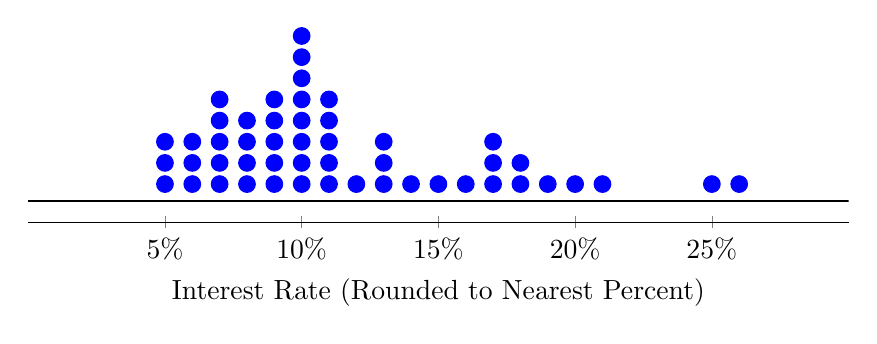
\begin{tikzpicture}
\pgfplotsset{ every non boxed x axis/.append style={x axis line style=-},
     every non boxed y axis/.append style={y axis line style=-}}
\begin{axis}[
width=12cm,
height=4cm,
xlabel={Interest Rate (Rounded to Nearest Percent)},
ylabel={},
yticklabels={},
axis y line=none,
axis x line=bottom,
xticklabel=\pgfmathprintnumber{\tick}\%,
xtick={5,10,15,20,25},
ymin=0,
ymax=9,
xmin=0,
xmax=30,
scatter/use mapped color={
 %draw=mapped color,
 fill=blue,
},
]
\addplot [domain=0:30]  {1};
\addplot[scatter, only marks, blue, scatter src=y, mark size=3pt]
coordinates
{
(11, 1.8)
(11, 2.8)
(11, 3.8)
(11, 4.8)
(11, 5.8)
(10, 1.8)
(10, 2.8)
(10, 3.8)
(10, 4.8)
(10, 5.8)
(10, 6.8)
(10, 7.8)
(10, 8.8)
(26, 1.8)
(9, 1.8)
(9, 2.8)
(9, 3.8)
(9, 4.8)
(9, 5.8)
(17, 1.8)
(17, 2.8)
(17, 3.8)
(6, 1.8)
(6, 2.8)
(6, 3.8)
(8, 1.8)
(8, 2.8)
(8, 3.8)
(8, 4.8)
(13, 1.8)
(13, 2.8)
(13, 3.8)
(5, 1.8)
(5, 2.8)
(5, 3.8)
(7, 1.8)
(7, 2.8)
(7, 3.8)
(7, 4.8)
(7, 5.8)
(25, 1.8)
(18, 1.8)
(18, 2.8)
(19, 1.8)
(14, 1.8)
(20, 1.8)
(15, 1.8)
(12, 1.8)
(16, 1.8)
(21, 1.8)
};
\end{axis}
\end{tikzpicture}
\end{center}
\end{example}
\end{frame}

\begin{frame}
\begin{definition}
A \textbf{parameter} is a numerical measurement describing some characteristic of a population.
\end{definition}\pause
\begin{definition}
A \textbf{statistic} is a numerical measurement describing some characteristic of a sample.
\end{definition}\pause
\begin{note}
Parameter and population both start with a \textquote{P.}\\Statistic and sample both start with a \textquote{S.}
\end{note}
\end{frame}

\begin{frame}
\begin{definition}
A \textbf{measure of center} is a value at the center or middle of a data set.
\end{definition}\pause

\begin{definition}
The \textbf{mean} of a set of data is the measure of center found by adding all the data values and dividing by the total number of data values.
\end{definition}\pause

\begin{note}
The mean is also known as the \textbf{average}.
\end{note}\pause

\begin{block}{Properties of the Mean}
\begin{itemize}
\item Sample means drawn from the same population tend to vary less than other measures of center.\pause
\item A disadvantage of the mean is that just one extreme value can change the value of the mean substantially.
\end{itemize}
\end{block}
\end{frame}

\begin{frame}
\begin{block}{Common Notation}
Sample statistics are usually represented by English letters, such as $\bar{x}$, while population parameters are usually represented by Greek letters, such as $\mu$.\pause
\vspace{-4mm}
{\renewcommand*{\arraystretch}{2.2}
\begin{equation*}
\begin{matrix}[ll]
\sum & \text{denotes the sum of a set of data values.} \\\pause
x & \text{is used as a placeholder for the variable of interest.} \\\pause
n & \text{represents the number of data values in a sample.} \\\pause
N & \text{represents the number of data values in a population.} \\\pause
\bar{x}=\dfrac{\sum x}{n} & \text{is the mean of a set of sample values.} \\\pause
\mu = \dfrac{\sum x}{N} & \text{is the mean of all values in a population.}
\end{matrix}
\end{equation*}}
\end{block}
\end{frame}

\begin{frame}
\begin{example}\label{verizon}
Suppose we measure the of data speeds of smartphones from the four major carriers. The table contains five data speeds, in megabits per second (Mbps), from this data set.

\begin{center}
\begin{tabular}{|l|ccccc|}\hline
\text{Carrier} & \text{Verizon} & \text{Verizon} & \text{Verizon} & \text{Verizon} & \text{Verizon}\\
\text{Mbps} & 38.5 & 55.6 & 22.4 & 14.1 & 23.1\\\hline
\end{tabular}
\end{center}\pause

The mean is 
\begin{equation*}
\bar{x} = \dfrac{\sum x}{n}\pause
= \dfrac{38.5 + 55.6 + 22.4 + 14.1 + 23.1}{5}\pause
= \dfrac{153.7}{5}\pause
 = 30.74~\text{Mbps}
\end{equation*}
\end{example}\pause

\begin{note}
Round statistics and parameters to one more decimal place than found in the data.
\end{note}
\end{frame}

\begin{frame}
\begin{note}
It is common to mark the mean on a dot plot.
\end{note}\pause

\begin{example}\label{mean_dotplot}
The mean of \texttt{interest\_rate} is: (Do not round the data values.)
\begin{equation*}
\bar{x}=
\dfrac{\tiny\left(\begin{array}{c}5.31\%+5.31\%+5.32\%+6.08\%+6.08\%+6.08\%+6.71\%+6.71\%+7.34\%\\+7.35\%+7.35\%+7.96\%+7.96\%+7.96\%+7.97\%+9.43\%+9.43\%+9.44\%\\+9.44\%+9.44\%+9.92\%+9.92\%+9.92\%+9.92\%+9.93\%+9.93\%+10.42\%\\+10.42\%+10.9\%+10.9\%+10.91\%+10.91\%+10.91\%+11.98\%+12.62\%\\+12.62\%+12.62\%+14.08\%+15.04\%+16.02\%+17.09\%+17.09\%+17.09\%\\+18.06\%+18.45\%+19.42\%+20\%+21.45\%+24.85\%+26.3\%\end{array}\right)}{50}=11.567\%
\end{equation*}\pause
\vspace{-6mm}
\begin{center}
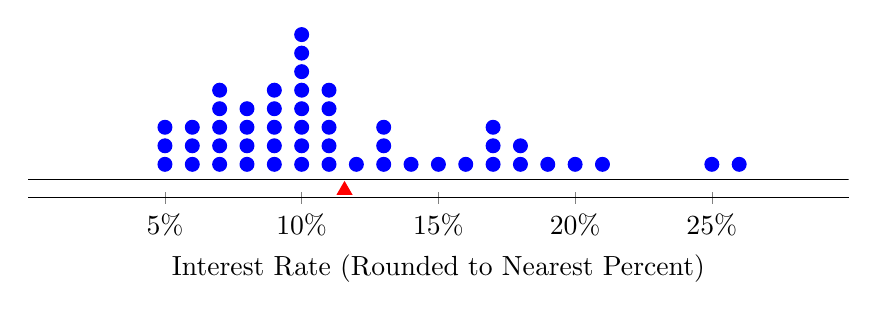
\begin{tikzpicture}
\pgfplotsset{ every non boxed x axis/.append style={x axis line style=-},
     every non boxed y axis/.append style={y axis line style=-}}
\begin{axis}[
width=12cm,
height=3.7cm,
xlabel={Interest Rate (Rounded to Nearest Percent)},
ylabel={},
yticklabels={},
axis y line=none,
axis x line=bottom,
xticklabel=\pgfmathprintnumber{\tick}\%,
xtick={5,10,15,20,25},
ymin=0,
ymax=9,
xmin=0,
xmax=30,
scatter/use mapped color={
 %draw=mapped color,
 fill=blue,
},
]
\addplot [domain=0:30]  {1};
\addplot[scatter, only marks, blue, scatter src=y, mark size=2.5pt]
coordinates
{
(11, 1.8)
(11, 2.8)
(11, 3.8)
(11, 4.8)
(11, 5.8)
(10, 1.8)
(10, 2.8)
(10, 3.8)
(10, 4.8)
(10, 5.8)
(10, 6.8)
(10, 7.8)
(10, 8.8)
(26, 1.8)
(9, 1.8)
(9, 2.8)
(9, 3.8)
(9, 4.8)
(9, 5.8)
(17, 1.8)
(17, 2.8)
(17, 3.8)
(6, 1.8)
(6, 2.8)
(6, 3.8)
(8, 1.8)
(8, 2.8)
(8, 3.8)
(8, 4.8)
(13, 1.8)
(13, 2.8)
(13, 3.8)
(5, 1.8)
(5, 2.8)
(5, 3.8)
(7, 1.8)
(7, 2.8)
(7, 3.8)
(7, 4.8)
(7, 5.8)
(25, 1.8)
(18, 1.8)
(18, 2.8)
(19, 1.8)
(14, 1.8)
(20, 1.8)
(15, 1.8)
(12, 1.8)
(16, 1.8)
(21, 1.8)
};
\addplot [scatter, only marks, red, scatter src=y, mark size=3pt, scatter/use mapped color={fill=red,}, mark=triangle*] coordinates {(11.567, 0.4)};
\end{axis}
\end{tikzpicture}
\end{center}
\end{example}
\end{frame}

\begin{frame}
\begin{example}
We saw in Example~\ref{mean_dotplot} that the average loan interest rate was 11.567\%.

\vspace{1mm}
\question{What is the mean of \textbf{all} loans in the country?}\pause
\answer{The best guess we can make is to use the sample mean of 11.567\%.}\pause

\vspace{2mm}
\question{Is this a good guess?}\pause
\answer{Just because the sample mean is the only educated guess we can make, doesn't mean it's anywhere close to the population mean.}
\end{example}\pause

\begin{definition}
A \textbf{point estimate} is a single value used to estimate a population parameter.
\end{definition}\pause

\begin{note}
We will discuss tools in Chapter 5 and beyond to determine how well a point estimate estimates a parameter.
\end{note}
\end{frame}

\begin{frame}
\begin{example}
We would like to determine if a new drug is more effective at treating asthma attacks than the standard drug. A trial of 1500 adults is setup, giving the following data.

\vspace{-5mm}
\begin{center}
\begin{tabular}{c|cc}
& New drug & Standard drug \\\hline
Number of patients & 500 & 1000 \\
Total asthma attacks & 200 & 300
\end{tabular}
\end{center}
\question{Can we conclude that the new drug is more effective?}\pause
\answer{Raw numbers can be deceptive when group sizes are unbalanced.}\pause
 
 \vspace{1mm}
Looking at the table, 200 is a smaller number than 300. \pause

\vspace{1mm}
But, when we calculate the means we get:

\vspace{-4mm}
\begin{center}
\begin{tabular}{lc}
New drug: & $200~\text{attacks} / 500~\text{patients}=0.4~\text{attacks per patient}$ \\[2mm]
Standard drug: & $300~\text{attacks} / 1000~\text{patients}=0.3~\text{attacks per patient}$
\end{tabular}
\end{center}\pause
The average number of asthma attacks per patient is higher with the new drug, so it's not more effective.
\end{example}
\end{frame}

\begin{frame}
\begin{example}
Emilio opened a food truck last year, and his business has stabilized over the last three months. During this three month period he made $\$11,000$, while working 625 hours.

\vspace{1mm}
\question{Is Emilo doing well with his new business?}\pause
\answer{If you haven't ran a food truck, it can be hard to tell if $\$11,000$ is a high amount or a low amount.}\pause

\vspace{1mm}
Calculating the mean gives:
\begin{equation*}
\dfrac{\$11000}{625~\text{hours}} = \$17.60~\text{per hour}
\end{equation*}
\end{example}\pause

\begin{note}
The mean gives a standardized a metric into something easier to interpret and compare.
\end{note}
\end{frame}

\begin{frame}
\begin{example}
Suppose we want to find the average income per person across the entire United States. To do so, we take the mean of the \texttt{per\_capita\_income} variable from the \texttt{county} data set.

\vspace{1mm}
\question{Is this the best approach?}\pause
\answer{No. Each county represents multiple people. If we computed the mean of \texttt{per\_capita\_income} we  would be treating a county with $5,000$ residents and a county with $5,000,000$ residents the same.}\pause

\vspace{1mm}
To account to differences in the population of each county, we should:
\begin{enumerate}
\item Calculate the total income for each county. {\small$\left(\texttt{pop2017}\times\texttt{per\_capita\_income}\right)$}\pause
\item Add up all the county income totals\pause
\item Then divide by the total number of people in the country.\pause
\end{enumerate}

Using this method we would find the average income per person in the US is $\$30,861$. If we had used the simple mean of \texttt{per\_capita\_income} the result would have been $\$26,093$, which is much lower.
\end{example}
\end{frame}

\begin{frame}
\begin{definition}
A \textbf{weighted mean} is a mean where some values contribute more than others. 
\begin{equation*}
\bar{x}=\dfrac{\sum w_x\cdot x}{\sum w_x}
\end{equation*}
The values $w_x$ are called the \textbf{weights}.
\end{definition}
\end{frame}

\begin{frame}
\begin{example}
Your final grade in this class is a weighted mean of the following four values:
\begin{center}
\begin{tabular}{l|c|c}
Value & \% of Grade & Weight \\\hline
Your average attendance score & 10\% & 10 \\\pause
Your average assignment score & 30\% & 30 \\\pause
Your average exam score & 40\% & 40 \\\pause
Your final exam score & 20\% & 20
\end{tabular}
\end{center}\pause
So, your final grade is calculated using the formula:
\begin{equation*}
\text{Grade} = \dfrac{10\cdot\overline{\text{attendance}} + 30\cdot\overline{\text{assignments}} + 40\cdot\overline{\text{exams}} + 20\cdot\text{final}}{10+30+40+20}
\end{equation*}
\end{example}\pause

\begin{note}
We could also use the decimal versions of the percentages as the weights, instead of the whole numbers.
\end{note}
\end{frame}

\begin{frame}
\begin{definition}
The \textbf{median} of a data set is the middle value when the original data values are arranged in order of smallest to largest.
\end{definition}\pause

\begin{block}{Properties}
\begin{itemize}
\item The median does not change by large amounts when we include an extreme value.
\end{itemize}
\end{block}\pause

\begin{block}{Notation}
The median of a sample is denoted $\tilde{x}$.
\end{block}\pause

\begin{block}{Procedure}
\begin{enumerate}
\item Sort the values.
\item 
\begin{itemize}
\item If the number of data values is odd, the median is the number located in the exact middle of the sorted list.
\item If the number of data values is even, the median is found by computing the mean of the two middle numbers in the sorted list.
\end{itemize}
\end{enumerate}
\end{block}
\end{frame}

\begin{frame}
\begin{example}
Let find the median data speed using the table from Example~\ref{verizon}.
\begin{center}
\begin{tabular}{|l|ccccc|}\hline
\text{Carrier} & \text{Verizon} & \text{Verizon} & \text{Verizon} & \text{Verizon} & \text{Verizon}\\
\text{Mbps} & 38.5 & 55.6 & 22.4 & 14.1 & 23.1\\\hline
\end{tabular}
\end{center}\pause

First sort the data values.
\begin{center}
\begin{tabular}{|ccccc|}\hline
14.1 & 22.4 & \textcolor<3->{blue}{23.1} & 38.5 & 55.6\\\hline
\end{tabular}
\end{center}\pause

We have 5 data values so the median is $\tilde{x} = \textcolor{blue}{23.1}$ Mbps.
\end{example}\pause

\begin{note}
This different than the mean 30.74 Mbps.
\end{note}
\end{frame}

\begin{frame}
\begin{example}
Let find the median data speed using the table from Example~\ref{verizon}, but with an extreme value added in.
\begin{center}
\begin{tabular}{|l|cccccc|}\hline
\text{Carrier} & \text{Verizon} & \text{Verizon} & \text{Verizon} & \text{Verizon} & \text{Verizon} & \text{Verizon} \\
\text{Mbps} & 38.5 & 55.6 & 22.4 & 14.1 & 23.1 & 192.6 \\\hline
\end{tabular}
\end{center}\pause

First sort the data values.
\begin{center}
\begin{tabular}{|cccccc|}\hline
14.1 & 22.4 & \textcolor<3->{blue}{23.1} & \textcolor<3->{blue}{38.5} & 55.6 & 192.6\\\hline
\end{tabular}
\end{center}\pause

We have 6 data values so $\tilde{x} = \dfrac{\textcolor{blue}{23.1}+\textcolor{blue}{38.5}}{2}=30.80$ Mbps.
\end{example}\pause

\begin{note}
This is very different from the mean of this table.
\begin{equation*}
\bar{x} = \dfrac{14.1+22.4+23.1+38.5+55.6+192.6}{6} = 173.15~\text{Mbps}
\end{equation*}
\end{note}
\end{frame}

\begin{frame}
\begin{definition}
A \textbf{histogram} is a graph consisting of bars of equal width drawn adjacent to each other. Each bar represents a \textquote{bin} of data values and the height of each bar is how many data values are in the \textquote{bin}.
\end{definition}\pause

\begin{block}{Important Uses}
\begin{itemize}
\item Visually displays the shape of the distribution of the data.\pause
\item Shows the location of the center of the data.\pause
\item Shows the spread of the data.\pause
\item Identifies extreme values.\pause
\end{itemize}
\end{block}

\begin{note}
Histograms are similar to dot plots, except that each bar represents a range of data values.
\end{note}
\end{frame}

\newcommand{\barcolor}[2]{\color<#1|handout:0>{red}{#2}}

\begin{frame}
\begin{example}
The table contains drive-through service times, in seconds.
\vspace{-2mm}
\begin{center}
\begin{tabular}{rrrrrrrrrrrr}
\barcolor{2}{107} & \barcolor{3}{139} & \barcolor{4}{197} & \barcolor{4}{209} & \barcolor{6}{281} & \barcolor{5}{254} & \barcolor{3}{163} & \barcolor{3}{150} & \barcolor{3}{127} & \barcolor{6}{308} & \barcolor{5}{206} \\
\barcolor{3}{169} &  \barcolor{2}{83} & \barcolor{3}{127} & \barcolor{3}{133} & \barcolor{3}{140} & \barcolor{3}{143} & \barcolor{3}{130} & \barcolor{3}{144} &  \barcolor{2}{91} &\barcolor{2}{113} & \barcolor{3}{153} \\
252 & \barcolor{4}{200} & \barcolor{2}{117} & \barcolor{3}{167} & \barcolor{3}{148} & \barcolor{4}{184} & \barcolor{2}{123} & \barcolor{3}{153} & \barcolor{3}{155} & \barcolor{3}{154} & \barcolor{2}{100} \\
\barcolor{2}{101} & \barcolor{3}{138} & \barcolor{4}{186} & \barcolor{4}{196} & \barcolor{3}{146} &  \barcolor{2}{90} & \barcolor{3}{144} &\barcolor{2}{119} & \barcolor{3}{135} & \barcolor{3}{151} & \barcolor{4}{197} \\
\end{tabular}
\end{center}
Let's build a histrogram:

\vspace{0mm}
\begin{center}
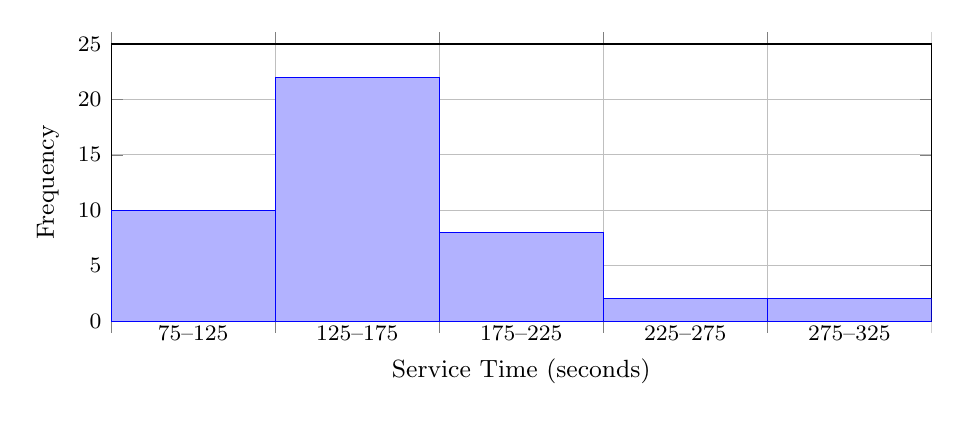
\begin{tikzpicture}
\begin{axis}[
small,
height=5.1cm,
width=12.0cm,
enlarge x limits=false,
enlarge y limits=false,
ybar interval,
ymajorgrids=true,
ylabel={Frequency},
xlabel={Service Time (seconds)},
x tick label style={rotate=0,anchor=center},
xtick={75, 125,...,325},
ytick={0,5,...,1000},
ymin=0,
ymax=25,
xmin=75,
xmax=325,
xticklabel style={/pgf/number format/.cd,fixed,precision=0},
xticklabel=
\pgfmathprintnumber\tick--\pgfmathprintnumber\nexttick,
]
\only<beamer:7|handout:1>{%
\draw [blue,fill=blue!30!white] (axis cs: 75,0) rectangle (axis cs: 125,10);
\draw [blue,fill=blue!30!white] (axis cs: 125,0) rectangle (axis cs: 175,22);
\draw [blue,fill=blue!30!white] (axis cs: 175,0) rectangle (axis cs: 225,8);
\draw [blue,fill=blue!30!white] (axis cs: 225,0) rectangle (axis cs: 275,2);
\draw [blue,fill=blue!30!white] (axis cs: 275,0) rectangle (axis cs: 325,2);
}
\temporal<2| handout:0>{\draw [style={opacity=0}] (axis cs: 75,0) rectangle (axis cs: 125,10);}%
                     {\draw [blue,fill=red] (axis cs: 75,0) rectangle (axis cs: 125,10);}%
                     {\draw [blue,fill=blue!30!white] (axis cs: 75,0) rectangle (axis cs: 125,10);}%
\temporal<3| handout:0>{\draw [style={opacity=0}] (axis cs: 125,0) rectangle (axis cs: 175,22);}%
                     {\draw [blue,fill=red] (axis cs: 125,0) rectangle (axis cs: 175,22);}%
                     {\draw [blue,fill=blue!30!white] (axis cs: 125,0) rectangle (axis cs: 175,22);}%
\temporal<4| handout:0>{\draw [style={opacity=0}] (axis cs: 175,0) rectangle (axis cs: 225,8);}%
                     {\draw [blue,fill=red] (axis cs: 175,0) rectangle (axis cs: 225,8);}%
                     {\draw [blue,fill=blue!30!white] (axis cs: 175,0) rectangle (axis cs: 225,8);}%
\temporal<5| handout:0>{\draw [style={opacity=0}] (axis cs: 225,0) rectangle (axis cs: 275,2);}%
                     {\draw [blue,fill=red] (axis cs: 225,0) rectangle (axis cs: 275,2);}%
                     {\draw [blue,fill=blue!30!white] (axis cs: 225,0) rectangle (axis cs: 275,2);}%
\temporal<6| handout:0>{\draw [style={opacity=0}] (axis cs: 275,0) rectangle (axis cs: 325,2);}%
                     {\draw [blue,fill=red] (axis cs: 275,0) rectangle (axis cs: 325,2);}%
                     {\draw [blue,fill=blue!30!white] (axis cs: 275,0) rectangle (axis cs: 325,2);}%
\end{axis}
\end{tikzpicture}
\end{center}
\end{example}
\end{frame}

\begin{frame}

\end{frame}
\end{document}
